\documentclass[6pt]{../../shared/AiTex}
\usepackage{csvsimple}
\usepackage{pdflscape}

\title{Memoria entrega 4}
\author{A.L.K.}
\date{Abril 2024}

\begin{document}
%\datos{facultad}{universidad}{grado}{asignatura}{subtitulo}{autor}{curso}
\datos{Informática}{Universidad Complutense de Madrid}{Ingeniería informática}{Aprendizaje Automatico y Big Data}{Entrega 6: diseño de redes neuronales}{Alejandro Barrachina Argudo}{2023-2024}
% \portadaApuntes
% \pagestyle{empty}
% \tableofcontents
% \pagestyle{empty}
\justify

\begin{center}

    {\huge \textbf{\underline{\subtitulo}}} \\
    { \lesson - \autor}

\end{center}


\section*{Introducción}

En este documento se explicará el código del entregable 6B y el proceso de diseño de redes neuronales con \textit{pytorch}.

Para esta práctica se usarán los siguientes \textit{imports} vistos en la figura \ref{fig:imports}. Parte del código se reutiliza de la práctica anterior.
\begin{figure}[H]
    \centering
    \lstinputlisting[firstline=1,lastline=11, style=custompython]{../evaluation.py}
    \caption{Código de las bibliotecas usadas}
    \label{fig:imports}
\end{figure}

También usaremos una serie de constantes para todo el programa (figura \ref{fig:constants}).

\begin{figure}[H]
    \centering
    \lstinputlisting[firstline=13,lastline=22, style=custompython]{../evaluation.py}
    \caption{Constantes del programa}
    \label{fig:constants}
\end{figure}

El \textit{dataset} para esta práctica lo generamos aleatoriamente con la función \textit{generate\_data} (figura \ref{fig:generate_data}). El dataset se compone de una linea de datos ``ideales'' y datos con ruido para comprobar la eficacia de la red neuronal.

Para dibujar estos datos usaremos la función \textit{plot\_data} (figura \ref{fig:plot_data}).

\begin{figure}[H]
    \centering
    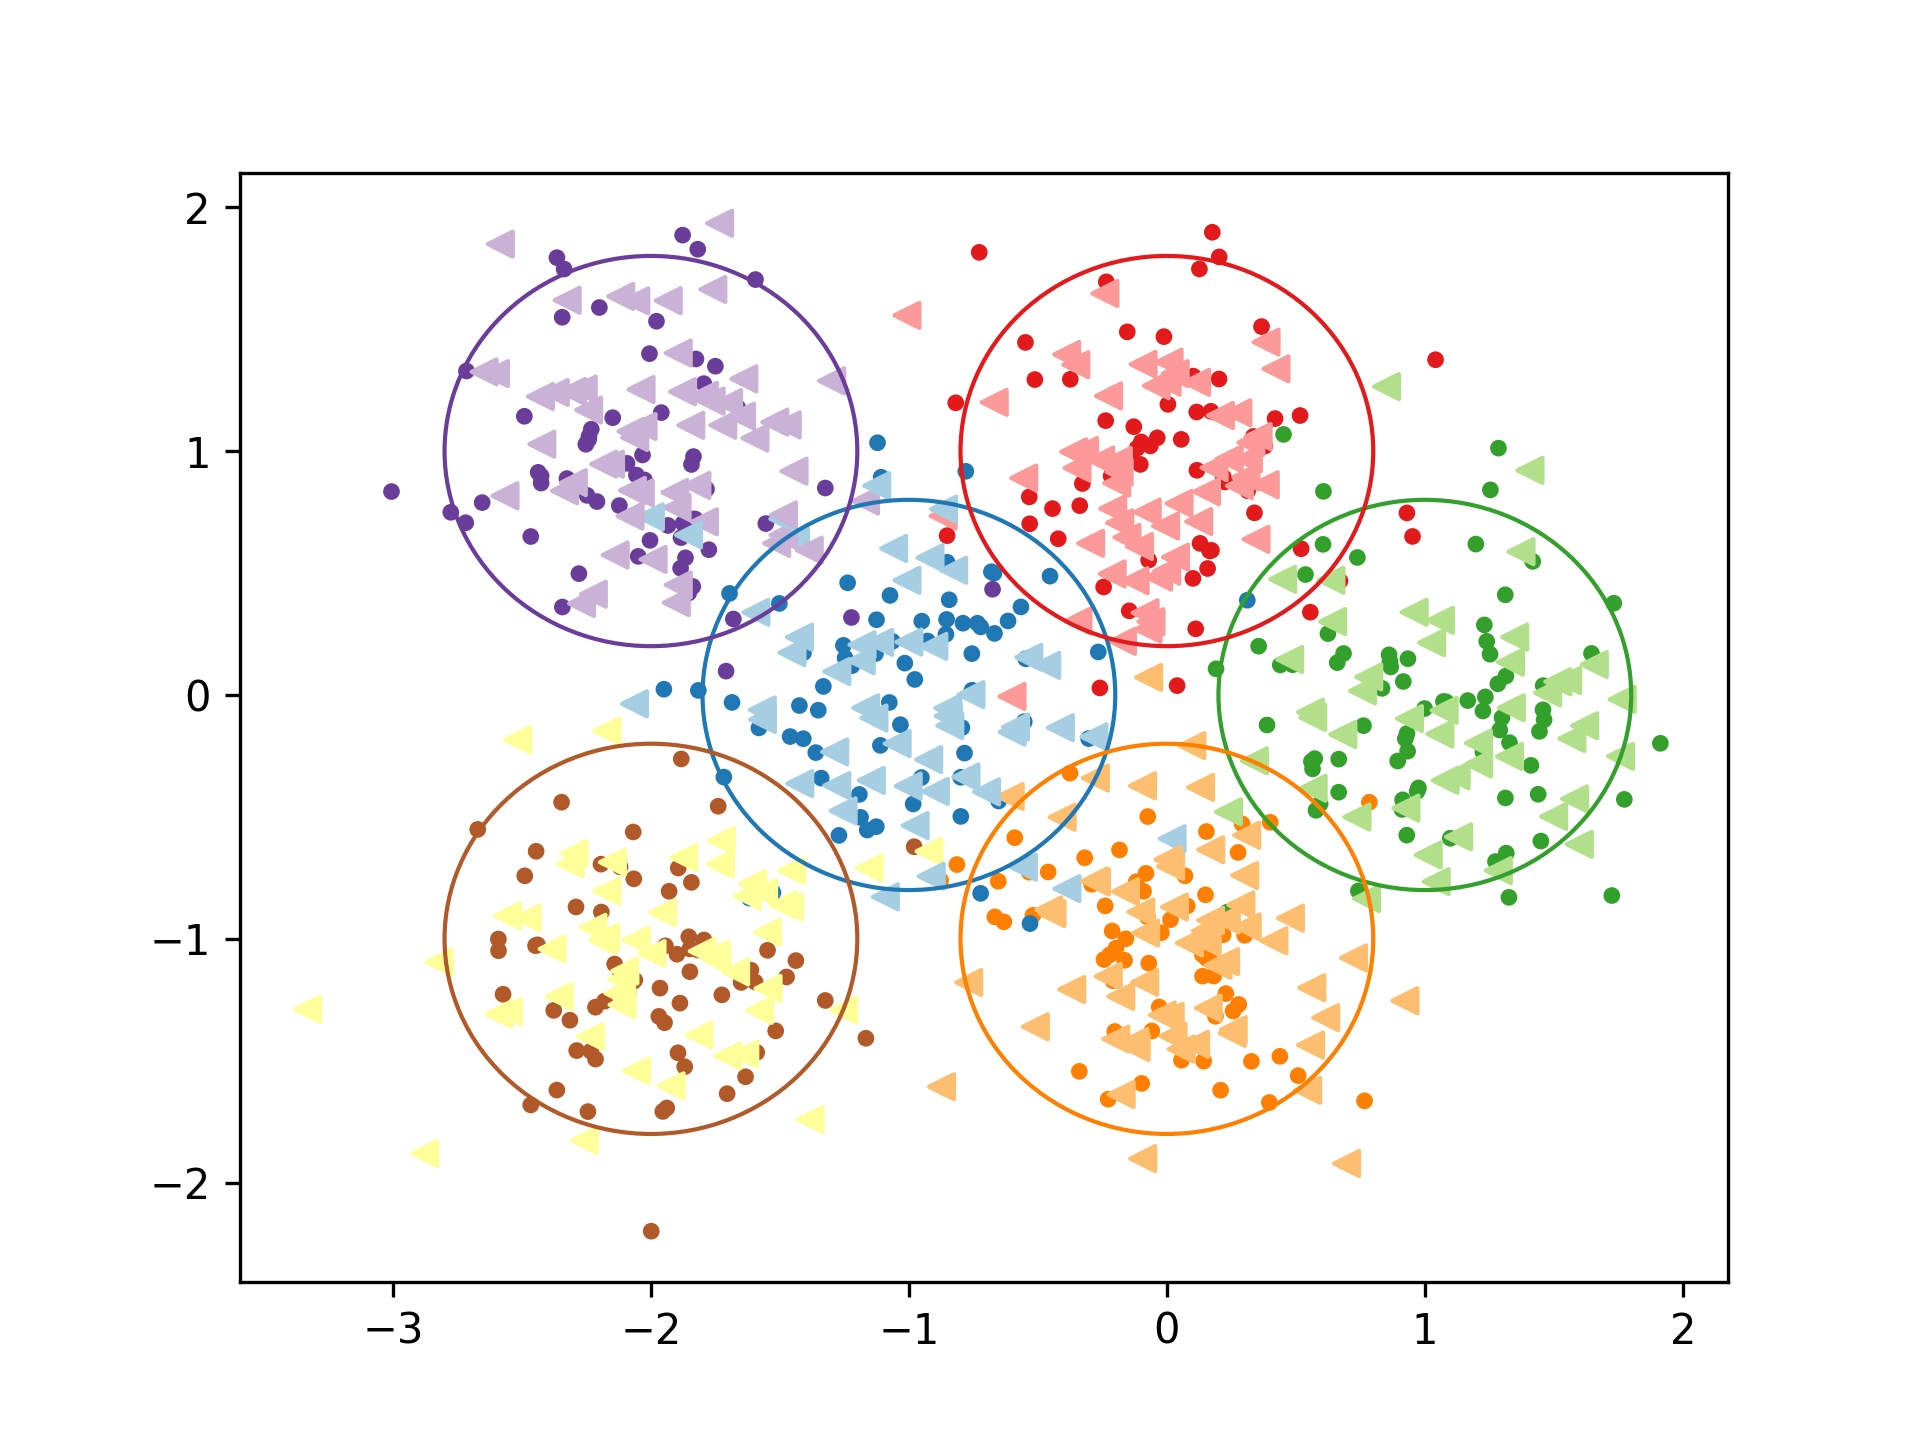
\includegraphics[width=0.5\textwidth]{./images/dataset.png}
    \caption{Ejemplo del \textit{dataset}}
    \label{fig:digitos}
\end{figure}

\begin{figure}[H]
    \centering
    \lstinputlisting[firstline=25,lastline=39, style=custompython]{../evaluation.py}
    \caption{Función \textit{generate\_data}}
    \label{fig:generate_data}
\end{figure}

\begin{figure}[H]
    \centering
    \lstinputlisting[firstline=287,lastline=307, style=custompython]{../evaluation.py}
    \caption{Función \textit{plot\_data}}
    \label{fig:plot_data}
\end{figure}

\section{Modelo complejo}

Usando \textit{pytorch} haremos un modelo complejo visto en la función \textit{ComplexModel()} (figura \ref{fig:complex_model}). Este modelo (y el resto) se componen usando la clase \textit{torch.nn.Sequential}. Las características de este modelo son:
\begin{itemize}
    \item Capa de 120 unidades y activación \textit{ReLu}
    \item Capa de 40 unidades y activación \textit{ReLu}
    \item Capa de 6 unidades y activación linear
\end{itemize}

Podemos ver los resultados en \textit{train} y \textit{cross-validation} en la figura \ref{fig:complex_results}. Para entrenar este modelo usaremos la función \textit{train\_model} (figura \ref{fig:train_model}) y las funciones \textit{train\_split} y \textit{train\_data}  (figuras \ref{fig:train_split} y \ref{fig:train_data})para preparar los datos para su procesado.

\begin{figure}[H]
    \centering
    \lstinputlisting[firstline=41,lastline=57, style=custompython]{../evaluation.py}
    \caption{Modelo complejo}
    \label{fig:complex_model}
\end{figure}

\begin{figure}[H]
    \centering
    \lstinputlisting[firstline=59,lastline=73, style=custompython]{../evaluation.py}
    \caption{Resultados del modelo complejo}
    \label{fig:complex_results}
\end{figure}

\begin{figure}[H]
    \centering
    \lstinputlisting[firstline=75,lastline=89, style=custompython]{../evaluation.py}
    \caption{Función \textit{train\_model}}
    \label{fig:train_model}
\end{figure}

\begin{figure}[H]
    \centering
    \lstinputlisting[firstline=91,lastline=105, style=custompython]{../evaluation.py}
    \caption{Función \textit{train\_split}}
    \label{fig:train_split}
\end{figure}

\section{Modelo simple}

\section{Modelo regularizado}

\section{Elegir el valor de regularización}

\section{Conclusiones}

\end{document}
